\documentclass{article}

\usepackage{amsmath}
\usepackage{amsfonts}
\usepackage{tikz}

\begin{document}
	
\author{Logan Grosz}
\title{Trapezoidal Rule}
\date{\today}

\maketitle

\begin{abstract}
\noindent The trapezoidal rule is a method of approximating an integral numerically. Because functions often is often curved, a trapezoid is more effective at approximating area under the curve than a rectangle, as found in a rectangular Riemann Sum.
\end{abstract}

\section{Declarations}

$a$; Upper limit of integral; $a\in \mathbb{R} $\\
$b$; Lower limit of integral; $b  \in \mathbb{R}$\\
$f$; Function that's integral is being approximated;\\
$n$; Number of subintervals for $\int f$ is being approximated; $n \in \mathbb{Z^+}$\\
$\Delta x$; x per n, also known as step size; $\Delta x \in \mathbb{R},\quad \Delta x = \frac{b-a}{n}$\\
$x_n$; x value at a certain n; $x_n = \Delta x \, n$

\section{Rule}

\begin{gather}
\intertext{Trapezoidal Rule:}
	T_n = \dfrac{1}{2} \Delta x (f(x_1) + 2\,f(x_2) + \,f(x_3) \cdots + 2\,f(x_{n-2}) + 2\,f(x_{n-1}) + f(x_n))
\end{gather}

\section{Pre-Derivation}
A trapezoid is a quadrilateral with two congruent side lengths and two variable side lengths.\\

\noindent The area of a trapezoid can be determined by finding the area of the subscribed rectangle via averaging the catheti.\\

\noindent Id Est\\
\begin{center}
	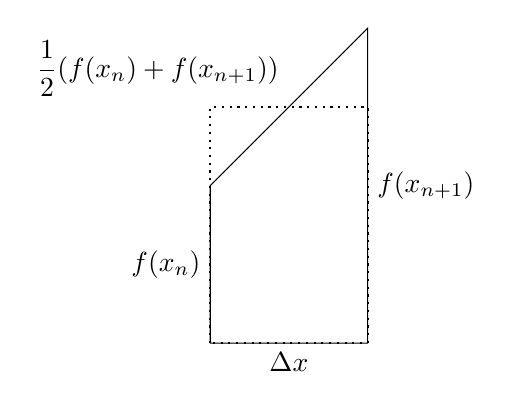
\begin{tikzpicture}
	%draw and label sides of trapezoid
	\draw (0,0) -- node[anchor=east] {$f(x_n)$} (0,2) -- (2,4) -- node[anchor=west] {$f(x_{n+1})$} (2,0) -- node[anchor=north] {$\Delta x$} (0,0);
	
	%draw subscribed rectangle
	\draw[thick, dotted] (0,0) -- (0,3) -- node[anchor=south east] {$\dfrac{1}{2}(f(x_n)+f(x_{n+1}))$} (2,3) -- (2,0) -- (0,0);
	\end{tikzpicture}
\end{center}

\noindent These trapezoids can be used to approximate the area under the curve of a function. See below.\\

\begin{center}
	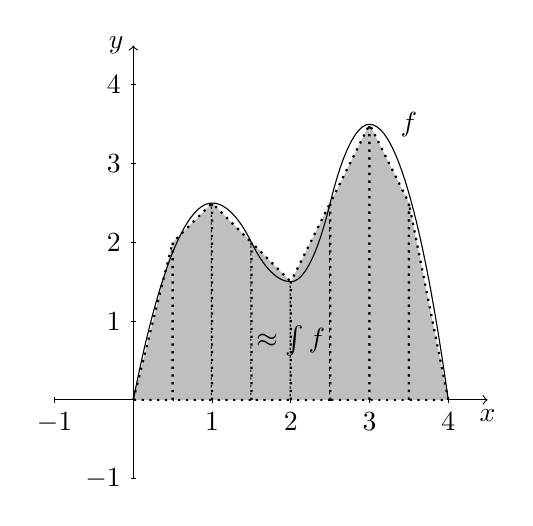
\begin{tikzpicture}
	%axis
	\draw[->] (0,-1) -- (0,4.5) node[at end,anchor=east]{$y$};
	\draw[->] (-1,0) -- (4.5,0) node[at end, anchor=north]{$x$};
	%x label
	\foreach \x in {-1,1,2,3,4}
	\draw (\x,1pt) -- (\x,-1pt) node[anchor=north] {$\x$};
	%y label
	\foreach \y in {-1,1,2,3,4}
	\draw (1pt,\y) -- (-1pt,\y) node[anchor=east] {$\y$};
	%trapezoid fillings
	\draw[thick,dotted,fill=lightgray] (0,0) -- (0,0) -- (0.5,2) -- (0.5,0) -- (0,0);
	\draw[thick,dotted,fill=lightgray] (0.5,0) -- (0.5,2) -- (1,2.5) -- (1,0) -- (0.5,0);
	\draw[thick,dotted,fill=lightgray] (1,0) -- (1,2.5) -- (1.5, 2.0) -- (1.5,0) -- (1,0);
	\draw[thick,dotted,fill=lightgray] (1.5,0) -- (1.5,2) -- (2,1.5) -- (2,0) -- (1.5,0);
	\draw[thick,dotted,fill=lightgray] (2,0) -- node{$\approx \int f$} (2,1.5) -- (2.5,2.5) -- (2.5,0) -- (2,0);
	\draw[thick,dotted,fill=lightgray] (2.5,0) -- (2.5,2.5) -- (3,3.5) -- (3,0) -- (2.5,0);
	\draw[thick,dotted,fill=lightgray] (3,0) -- (3,3.5) -- (3.5,2.5) -- (3.5,0) -- (3,0);
	\draw[thick,dotted,fill=lightgray] (3.5,0) -- (3.5,2.5) -- (4,0) -- (4,0) -- (3.5,0);
	%Parabola drawing
	\draw (0,0) parabola bend (1,2.5) (1.5,2);
	\draw (1.5,2) parabola bend (2,1.5) (2.5,2.5);
	\draw (2.5,2.5) parabola bend (3,3.5) (4,0);
	\node (function label) at (3.5,3.5){$f$};
	\end{tikzpicture}
\end{center}

\noindent The image above is a quartic function with eight subscribed trapezoids. Notice the error between the approximation and the actual area under the curve.

\section{Derivation}

\noindent The trapezoidal sum of the above image can be written as:

\begin{align*}
T_8=\frac{1}{2}\Delta x \, (f(x_1)+f(x_2)) &+ \frac{1}{2}\Delta x \, (f(x_2)+f(x_3))\\
   +\frac{1}{2}\Delta x \, (f(x_3)+f(x_4)) &+ \frac{1}{2}\Delta x \, (f(x_4)+f(x_5))\\
   +\frac{1}{2}\Delta x \, (f(x_5)+f(x_6)) &+ \frac{1}{2}\Delta x \, (f(x_6)+f(x_7))\\
   +\frac{1}{2}\Delta x \, (f(x_7)+f(x_8))
\end{align*}

\noindent A generalized form of this equation can be written as:

\begin{align*}
T_n&=\frac{1}{2}\Delta x \, (f(x_1)+f(x_2)) + \frac{1}{2}\Delta x \, (f(x_2)+f(x_3))\\
   &+\frac{1}{2}\Delta x \, (f(x_3)+f(x_4)) + \frac{1}{2}\Delta x \, (f(x_4)+f(x_5))\\
   \vdots\\
   &+\frac{1}{2}\Delta x \, (f(x_{n-3})+f(x_{n-2})) + \frac{1}{2}\Delta x \, (f(x_{n-2})+f(x_{n-1}))\\
   &+\frac{1}{2}\Delta x \, (f(x_{n-1})+f(x_n))\\
\end{align*}

\noindent By diving out common factors:

\begin{align*}
T_n&=\frac{1}{2}\Delta x (f(x_1) + f(x_2) + f(x_2) + f(x_3)\\
					   &+ f(x_3) + f(x_4) + f(x_4) + f(x_5)\\
					   &\vdots\\
					   &+ f(x_{n-3}) + f(x_{n-2}) + f(x_{n-2})\\
					   &+ f(x_{n-1}) + f(x_{n-1}) + f(x_{n}))
\end{align*}

\noindent By combining like terms:

\begin{align*}
T_n=\frac{1}{2}\Delta x(f(x_1)+2\,f(x_2)+2f(x_3)\cdots+2\,f(x_{n-2})+2\,f(x_{n-1})+f(x_n))
\end{align*}

\section{Exempli Gratia}

Examples of important instances

\end{document}